%%% License: Creative Commons Attribution Share Alike 4.0 (see https://creativecommons.org/licenses/by-sa/4.0/)
%%% Slides are based heavily on earlier versions of this course taught by Jesper Rudiger.

\documentclass[english,10pt]{beamer}
\DeclareGraphicsExtensions{.eps, .pdf,.png,.jpg,.mps,}
\usetheme{reMedian}
\usepackage{parskip}
\makeatother

\renewcommand{\baselinestretch}{1.2} 

\usepackage{amsmath, amssymb, amsfonts, amsthm}
\usepackage{enumerate}
\usepackage{hyperref}
\usepackage{url}
\usepackage{bbm}
\usepackage{color}

\usepackage{tikz}
\usepackage{tikzscale}
\newcommand*\circled[1]{\tikz[baseline=(char.base)]{
\node[shape=circle,draw, inner sep=-20pt] (char) {#1};}}
\usetikzlibrary{automata,positioning}
\usetikzlibrary{decorations.pathreplacing}
\usepackage{pgfplots}
\usepgfplotslibrary{fillbetween}
\usepackage{graphicx}

\usepackage{setspace}
\thinmuskip=1mu
\medmuskip=1mu 
\thickmuskip=1mu 

\theoremstyle{definition} 
\newtheorem{thm}{Theorem}
\newtheorem{claim}{Claim}
\newtheorem{proposition}{Proposition}
\usecolortheme{default}
\usepackage{verbatim}
\usepackage[normalem]{ulem}
\usepackage{appendixnumberbeamer}



\title{Financial Markets Microstructure \\ Lecture 2}

\subtitle{Measuring Liquidity \\
Chapter 2 of FPR}

\author{Egor Starkov}

\date{K{\o}benhavns Unversitet \\
	Spring 2020}



\begin{document}
\frame[plain]{\titlepage}
\addtocounter{framenumber}{-1}


\section{Revision}

\begin{frame}{Today on FMM:}
	\tableofcontents[currentsection]
\end{frame}


\begin{frame}{What did we do last week?}
	\begin{enumerate}
		\item Introduce financial markets broadly speaking and motivate why we wanted to talk about it
		\item Compare to classic `Walrasian' markets
		\begin{itemize}
			\item In financial markets, traders are normally strategic (i.e. not price takers) and timing matters
			\item Thus, markets may not be efficient: enter policy
		\end{itemize}
		\item Introduce some of the key concepts and language: dealer sets bid/ask price, market/limit order
		\item Categorize the most important types of institutions:  order-driven markets (auctions)/dealer markets
		\item Think about issues: bubbles, role of public/private information, policy
	\end{enumerate}
\end{frame}


\begin{frame}{Problems from last time}
	\begin{itemize}
		\item Find bid and ask prices for Facebook shares and for Microsoft. Which stock exchange do they come from? 
		%NOTE: FB listed on NASDAQ, BMV Mexico, and Xetra (Frankfurt); Microsoft on NASDAQ, SIX Swiss Ex, and Vienna
		\item Exercises 1-3 on pages 44-45 in the textbook - Friday
	\end{itemize}
\end{frame}


\begin{frame}{Today}
	\begin{itemize}
		\item Liquidity: why do we care?
		\item How can we measure it?
		\item What data problems are there? How can we get around these to measure liquidity?
		\item What do we typically find?
	\end{itemize}
\end{frame}


\section{Liquidity}

\begin{frame}{Today on FMM:}
	\tableofcontents[currentsection]
\end{frame}


\begin{frame}{Liquidity}
\begin{itemize}
	\item \alert{Market liquidity} = ``market's ability to facilitate an asset being sold quickly without having to reduce its price very much (or even at all)''
	\item Do not confuse with (related notions of):
\end{itemize}
\begin{enumerate}
	\item \structure{Funding liquidity} = ``economic agent's ability to obtain cash/credit at acceptable terms, to meet obligations without incurring large losses''
	\begin{itemize}
		\item Banks are `liquidity constrained' when they do not have enough cash on hands to meet demand for withdrawals (despite having enough assets)
		\item You are liquidity constrained when your wage arrives in two days but you need to pay your rent today.
	\end{itemize}
	\item \structure{Monetary liquidity} = ``asset's ability to be exchanged for goods''
	\begin{itemize}
		\item Assets in the order of decreasing liquidity: cash, checking deposits, long-term deposits, housing, ...
	\end{itemize}
\end{enumerate}
%\end{itemize}
\end{frame}


\begin{frame}{Importance of Liquidity}
\begin{itemize}
	\item Traders: liquidity provides a measure of trading costs
	\item Why important to the rest of us?
	\begin{enumerate}
		\item Efficiency is tricky to measure in financial markets: liquidity provides a proxy
		\item Illiquidity \textit{may} be a sign of structural problems in the market
		\item Illiquid markets also seem to be more prone to medium-run price deviations from fundamentals
	\end{enumerate}
	\item Relation to depth: depth measures how much must be traded to move price by certain amount
\end{itemize}
\end{frame}


\begin{frame}{Liquidity dry ups}
	Liquidity can dry up in the face of adverse events
	\begin{center}
		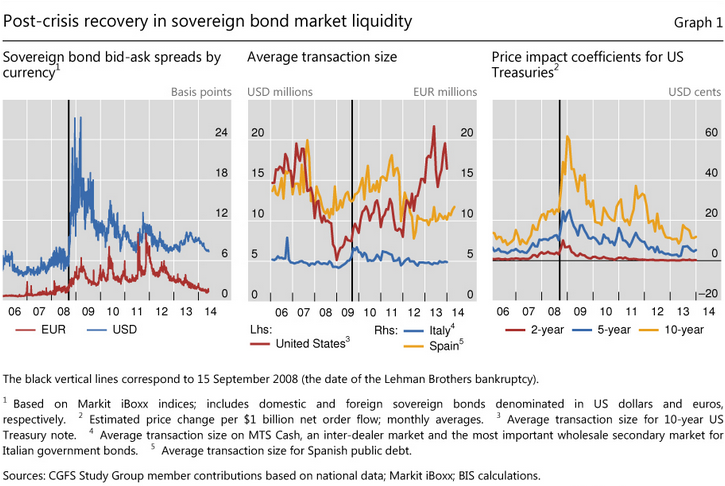
\includegraphics[scale=0.4]{pics/L2_liquiditylehman}
	\end{center}
\end{frame}


\begin{frame}{Liquidity measures}
	There is not a unique measure of liquidity -- today we will consider several:
	\begin{enumerate}
		\item \textbf{Spread measures}: quoted spread, effective spread, realized spread
		\item \textbf{Volume-weighted average price}: simply using average prices
		\item \textbf{Price impact}: How much does the price move after a trade
		\item \textbf{Non-trading measures}: trading volumes
	\end{enumerate}

	When trade direction is not available: estimate via \structure{Lee-Ready algorithm}. 
	
	When quote data are not available: estimate them using \structure{Roll's measure}
\end{frame}



\section{Measures of Liquidity}

\begin{frame}{Today on FMM:}
	\tableofcontents[currentsection]
\end{frame}


\begin{frame}{Example}
	\begin{itemize}
		\item Consider the following bid/ask/realized prices on KrispyKreme stock
		\begin{center}
			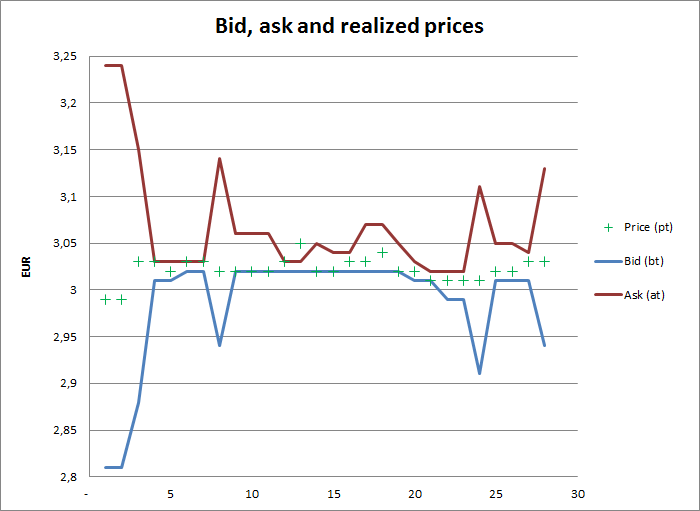
\includegraphics[scale=0.34]{pics/L2_bidask}
		\end{center}
		\item Notice that price is sometimes inside spread: price improvements (either hidden limits orders or price improvement given by dealer)
		\item Also a price outside spread (recall bid/ask only valid for x units)
	\end{itemize}
\end{frame}


\begin{frame}{Example (2)}
	\begin{itemize}
		\item Add \textit{trade direction}, i.e. whether trade was initiated by buyer/seller
		\begin{center}
			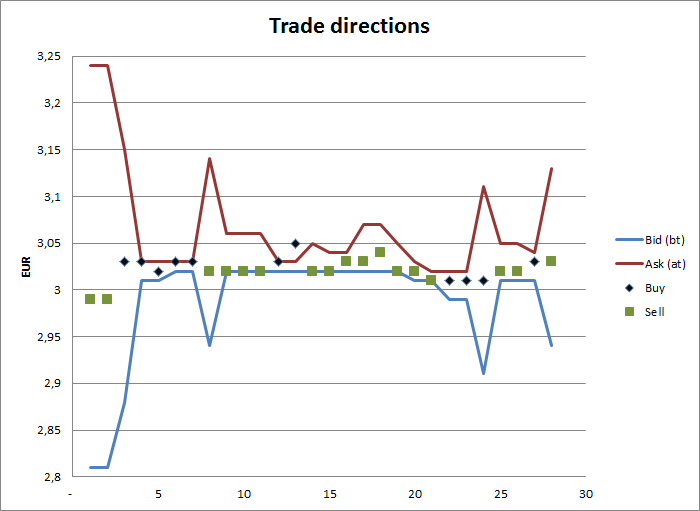
\includegraphics[scale=0.39]{pics/L2_directions}
		\end{center}
	\end{itemize}
\end{frame}


\begin{frame}{Quoted spread}
	\begin{itemize}
		\item \textbf{Contemporaneous}: spread facing trader at time $t$
		\item Let $a_t$ ($b_t$) be the best ask (bid) price at time $t$
		\item \alert{Quoted spread}:
		\[
		S_t = a_t -b_t
		\]
		\item Normalize to get \structure{normalized quoted spread}
		\[
		s_t = \frac{S_t}{m_t},
		\]
		where $m_t$ is the midprice:
		\begin{center}
			$
			m_t = \frac{a_t+b_t}{2}.
			$
		\end{center}
		\item We can generalize it to consider average spread for trade size $q$: 
		\begin{center}$S_t(q)=\overline{a}_t(q)-\overline{b}_t(q)$\end{center}
		where $\overline{a}_t(q)$ and $\overline{b}_t(q)$ are average execution prices
	\end{itemize}
\end{frame}


\begin{frame}{Quoted spread}
	\begin{itemize}
		\item Applying the definition to the data, we get:
		\begin{center}	
			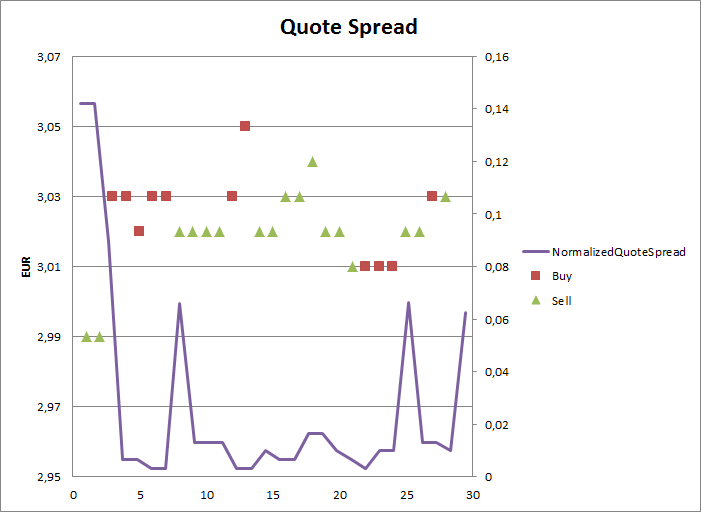
\includegraphics[scale=0.35]{pics/L2_quotespread}
		\end{center}
		\item Notice that the quoted spread does not capture price improvements (for instance in the first three observations)
	\end{itemize}
\end{frame}


\begin{frame}{Effective spread}
	\begin{itemize}
		\item \textbf{Backward looking}: spread faced by previous trader
		\item Suppose one market order is executed per period, and
		\begin{itemize}
			\item $d_t$: trade direction (1: buyer-initiated, -1: seller initiated)
			\item $p_t$:  price
		\end{itemize}
		\item \alert{Effective spread}: 
		\begin{align*}
		S^e_t & = d_t(p_t-m_{t}), \\
		s^e_t & = \frac{S^e_t}{m_{t}}
		\end{align*}
		\item Compare actual price with midquote the instant before: measures price impact and captures `price improvements'
	\end{itemize}
\end{frame}


\begin{frame}{Effective spread}
	\begin{itemize}
		\item Apply to data and compare to quoted spread
		\begin{center}
			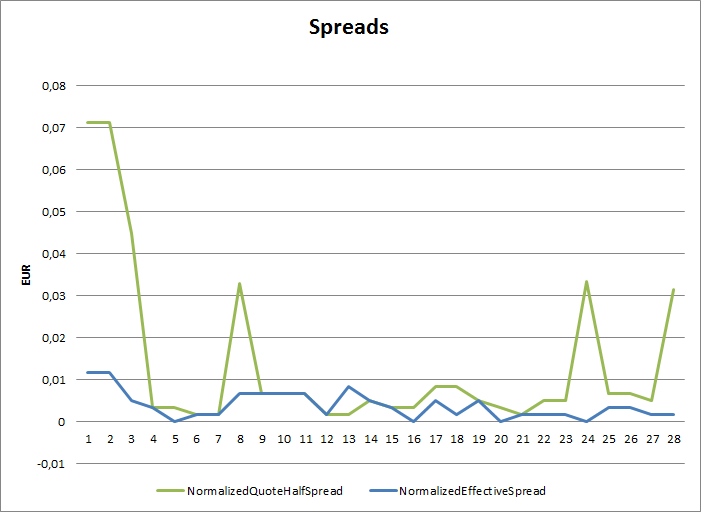
\includegraphics[scale=0.39]{pics/L2_effectivespread}
		\end{center}
		\item Effective spread is often lower (since it captures price improvements)
	\end{itemize}
\end{frame}


\begin{frame}{Realized spread}
	\begin{itemize}
		\item \textbf{Forward looking}: spread realized by somebody who holds the asset for $\Delta$ periods
		\item \alert{Realized spread}:
		\begin{align*}
		S^r_t & = d_t(p_t - m_{t+\Delta}) \\
		& = d_t(p_t-m_t) - d_t(m_{t+\Delta}-m_t)
		\end{align*}
		\item Idea: measure the spread after prices have adjusted to new information
		\item Typically smaller than effective spreads: why?
	\end{itemize}
\end{frame}


\begin{frame}{Realized spread}
	\begin{itemize}
		\item Calculate for $\Delta=5$ and compare to other measures
		\begin{center}
			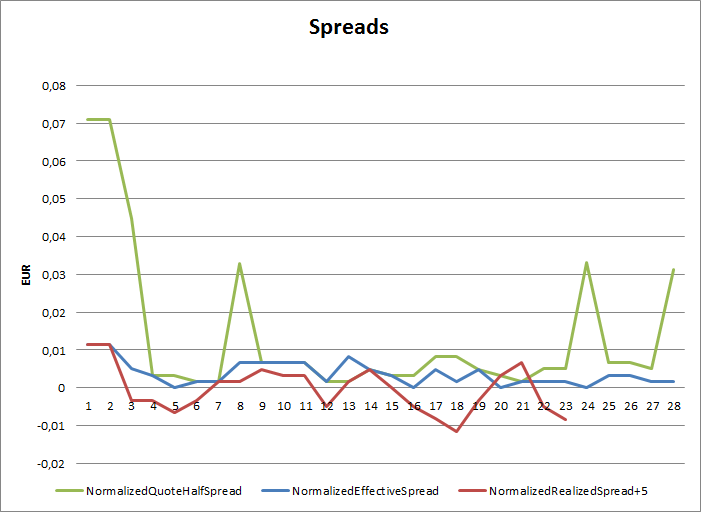
\includegraphics[scale=0.39]{pics/L2_realizedspread}
		\end{center}
		\item Realized spread is indeed often lower than effective spread
	\end{itemize}
\end{frame}


\begin{frame}{Comparing the spreads}
	\begin{itemize}
		\item The \structure{quoted spread} and the \structure{effective spread} may be more useful to traders:
		\begin{itemize}
			\item Quoted spread: what is the quoted trading cost now 
			\item Effective spread: what was the trading cost faced by the last trader
		\end{itemize}
		These are (imperfect) measures of the cost of executing a market order now
		\item The \structure{realized spread} is more relevant to a market maker (liquidity provider):
		\begin{itemize}
			\item It measures the cost of taking a position (long or short) for an amount of time
		\end{itemize}
	\end{itemize}
\end{frame}


\begin{frame}{Estimating direction of trade}
	\begin{itemize}
		\item We often only observe quotes and realized prices: not the direction of trade
		\item Thus, we need to develop methods to classify trades
		\item Complication: trading may be `within the quotes': harder to guess direction
		\item \alert{Lee-Ready algorithm}:
		\[
		d_t = \left\{
		\begin{aligned}
		1 & \text{ if } |p_t-a_t| < |p_t-b_t| \\
		&\text{ or } p_t=m_t \text{ and } p_t>p_{t-1}\\
		-1 & \text{ if } |p_t-a_t| > |p_t-b_t| \\
		& \text{ or } p_t=m_t \text{ and } p_t<p_{t-1} \\
		\end{aligned}
		\right.
		\]
	\end{itemize}
\end{frame}


\begin{frame}{Estimating Lee-Ready}
	First, we calculate midprices and compare to trade prices
	\center
	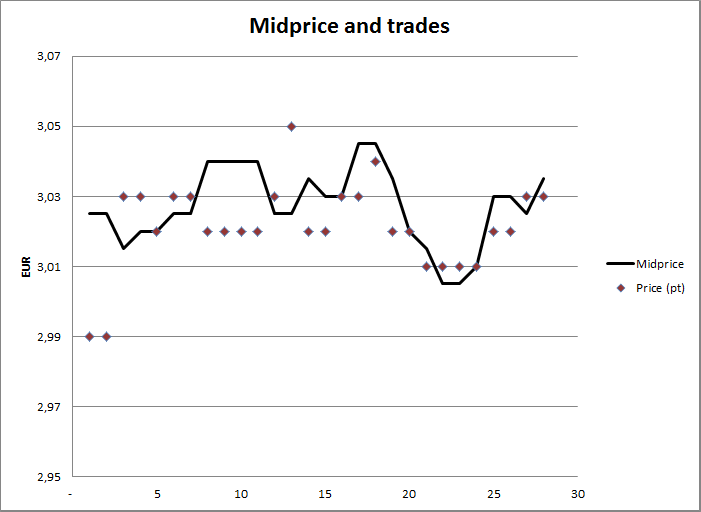
\includegraphics[scale=0.39]{pics/L2_midandtrade}
\end{frame}


\begin{frame}{Estimating Lee-Ready (2)}
	Then we compare trade prices to midprices
	\center
	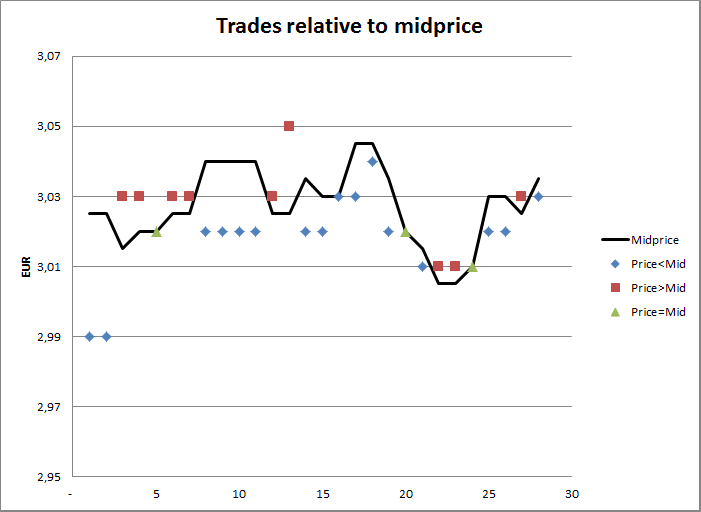
\includegraphics[scale=0.39]{pics/L2_traderelativemid}
\end{frame}


\begin{frame}{Estimating Lee-Ready (3)}
	Finally, we classify the trades that were just on the midprice
	\center
	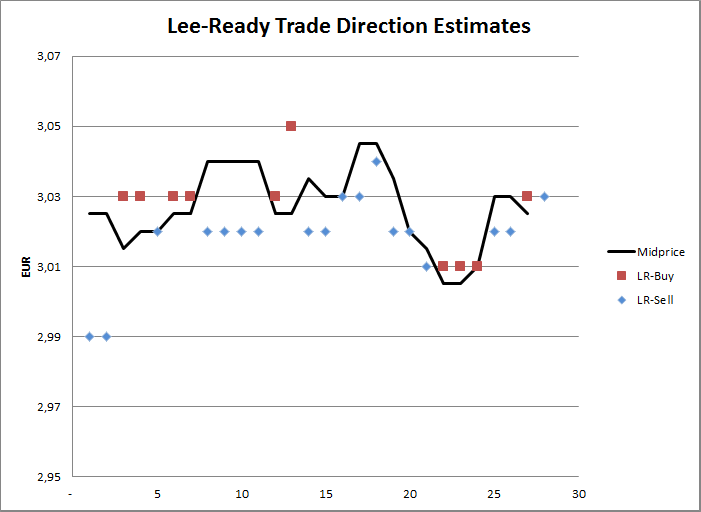
\includegraphics[scale=0.39]{pics/L2_leereadyest}
	%TODO: look up whether this is done at random or somehow else
\end{frame}


\begin{frame}{Estimating Lee-Ready (4)}
	Checking with the actual trade directions, we see that we only made one mistake
	\center
	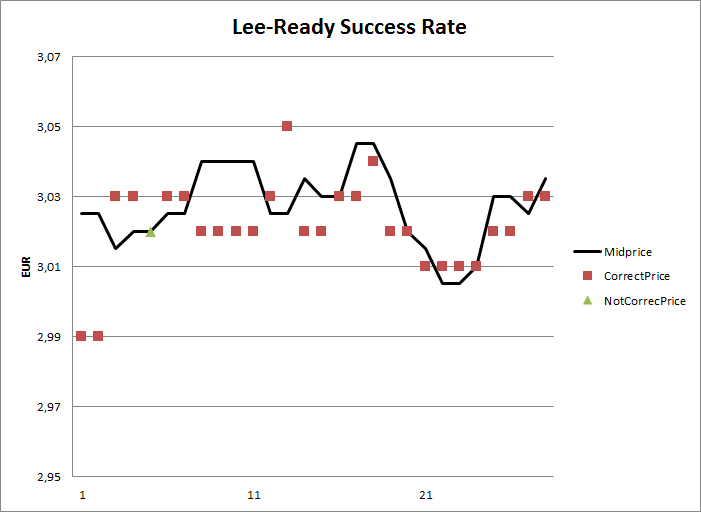
\includegraphics[scale=0.39]{pics/L2_leereadysuccess}
\end{frame}


\begin{frame}{Volume based measure}
	\begin{itemize}
		\item Let $q_t$ be the order imbalance (net market purchase)
		\item \alert{Volume-Weighted Average Price} (VWAP):
		\[
		VWAP = \sum  w_t p_t,
		\]
		where $w_t = |q_t|/\sum |q_t|$ is the order weight
		\item  This equals the amount of dollars traded over the number of shares traded: average price
		\item This measure may depend excessively on few orders (if they are large) and therefore be subject to manipulation
		\item For our example, $VWAP=3.02$
	\end{itemize}
\end{frame}


\begin{frame}{Price impact}
	\begin{itemize}
		\item How much do trades affect prices? We can estimate this by
		\[
		\Delta m_t = \lambda q_t + \epsilon_t.
		\]
		In our example: $\lambda = 0.15 $ ($q_t$ in 100,000EUR)
		\item  $\lambda$ captures price impact;  $1/\lambda$ captures market \textit{depth}
		\item Hasbrouck: sensitivity of returns to trading volume
		\[
		|\Delta m_t | = \gamma Vol_t + \epsilon_t.
		\]
		In our example: $\gamma = 0.01$ ($Vol_t$ in 100,000EUR)
		\item Amihud: take ratio btw return $r_t$ and volume to get \textit{illiquidity ratio}: 
		\center
		$I_t = \frac{|r_t|}{Vol_t}$.
	\end{itemize}
	%TODO: look up
\end{frame}


\begin{frame}{Amihud's Illiquidity Ratio}
	\center
	\includegraphics[scale=0.39]{pics/L2_Amihud}
\end{frame}


\begin{frame}{Other measures}
	\begin{itemize}
		\item Measures such as trading volume, turnover rate, trade frequency are also used
		\item Problem: trading volume and spreads are both positively correlated with information releases (think about why this is?)
		\item Frequency of trading or related measures may be more relevant in `thin' markets, for instance in emerging economies
	\end{itemize}
\end{frame}



\section{Estimating quotes}

\begin{frame}{Today on FMM:}
	\tableofcontents[currentsection]
\end{frame}


\begin{frame}{Quote data}
	\begin{itemize}
		\item We often lack information to compute the spread
		\item Roll: use transaction prices to estimate it
		\begin{enumerate}
			\item Construct a simple model of trading and calculate spread
			\item Estimate it
			\item Check robustness to simplifying assumptions
		\end{enumerate}
		\item Roll's estimator can almost always be computed
	\end{itemize}
\end{frame}


\begin{frame}{Roll's model}
	Suppose the following:
	\begin{enumerate}
		\item All trades have the same size. $d=1$: buy, $d=-1$: sell
		\item Arriving orders are i.i.d. with $\mathbb{P}(d_t =1)=\frac{1}{2}$
		\item Midquote is random walk: $m_t -m_{t-1} = \epsilon_t$  , where $\epsilon_t$ are i.i.d. shocks
		\item Market orders are not informative: $\mathbb{E}(d_t \epsilon_t)=\mathbb{E}(d_t \epsilon_{t+1})=0$
	\end{enumerate}
	Let $S = a_t-b_t$. Then
	\[
	p_t = m_t + \frac{d_t S}{2}.
	\]
	We know $p_t$ but not $m_t$. How do we estimate $S$?
\end{frame}


\begin{frame}{Roll's model}
	\begin{itemize}
		\item Roll's observed that although $\epsilon_t$ and $d_t$ are i.i.d., $\Delta d_t$ is mean-reverting:
		\begin{align*}
		Cov(\Delta d_t, \Delta d_{t-1})	= -1
		\\
		\\
		\\
		\\
		\\
		\end{align*}
		\item Intuitively: $\Delta d_t>0$ means that we go from a sale to a buy - the next change must be opposite
	\end{itemize}
\end{frame}


\begin{frame}{The estimator}
	\begin{itemize}
		\item We can then work out that
		\[
		Cov(\Delta p_t, \Delta p_{t-1}) = - \frac{S^2}{4},
		\]
		giving us the estimator
		\[
		S^R_t = 2 \sqrt{-Cov(\Delta p_t, \Delta p_{t-1})}.
		\]
		\item Recall the assumptions of the model. We (the book) can work out extensions to treat each of them
		\item In our example: $S^R_t = 0.01$
		\item Which of the previous spreads is Roll's estimator most affine to?
	\end{itemize}
\end{frame}


\begin{frame}{Implementation shortfall}
	\begin{itemize}
		\item The previous measures the time it takes to execute order %TODO - ???
		\item Aim at time 0: to (net) purchase $q$ shares
		\begin{itemize}
			\item By time $t$, fraction $\kappa_t$ has been executed, at an average execution price $\bar{p}_t$
			\item The realized trading gain is $\kappa_t q(m_t-\bar{p}_t)$
			\item An ideal gain from immediate execution without price impact would have been $q(m_t - m_0)$
			\item The difference is the \alert{implementation shortfall}:
			\begin{align*}
			IS_t 
			& = q(m_t-m_0) - \kappa_t q (m_t - \bar{p}_t) \\
			& = \kappa_t q(\bar{p}_t - m_0) + (1-\kappa_t) q (m_t - m_0).
			\end{align*}
			\item Interpretation: Execution cost plus opportunity cost
		\end{itemize}
	\end{itemize}
\end{frame}



\begin{frame}{Implementation shortfall}
	In the example... 
	\begin{itemize}
		\item Suppose you want to buy 3,500 shares
		\item And suppose all the buy orders come from you
	\end{itemize}
	\center
	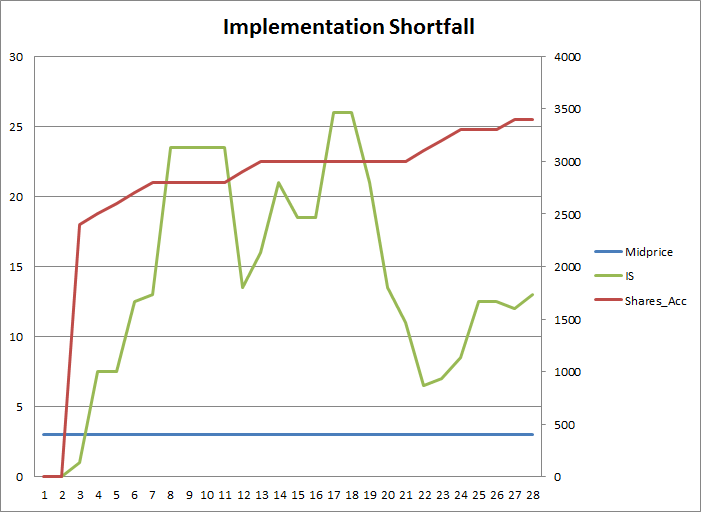
\includegraphics[scale=0.39]{pics/L2_is}
\end{frame}


\begin{frame}{Implementation shortfall (2)}
	Breaking down the shortfall into opportunity cost and execution cost
	\center
	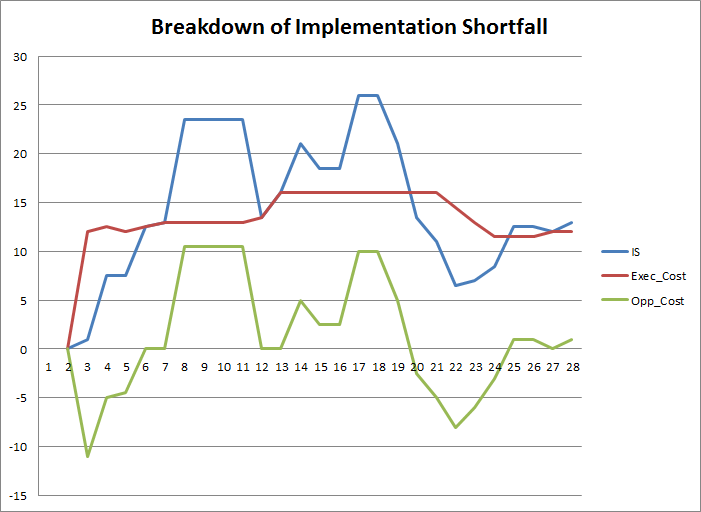
\includegraphics[scale=0.39]{pics/L2_is2}
\end{frame}


\begin{frame}{Conclusion}
	\begin{itemize}
		\item We have looked at different manners in which to estimate liquidity
		\item No method is perfect: depends on trade size, time horizon, trade motivation
		\item Data shows that liquidity varies both continuously throughout a trading day, and more abruptly around big events
		\item Next time we will start analyzing \textit{what} drives the spread
	\end{itemize}
\end{frame}


\begin{frame}{Exercises for next week}
	\begin{itemize}
		%\item In Absalon, I have attached a commission and fee schedule from Robinhood Financial. More information on \url{www.robinhood.io/}. Discuss the potential effect on other brokerage services.
		\item Recreate the graphs and figures I presented today using the KrispyKreme dataset
		\item Solve exercise 8 regarding implementation shortfall, on page 75 in the textbook.
		Discuss the meaning of $m_t$ in this analysis. 
		%TODO: bad ambiguous problem, consider replacing
	\end{itemize}
\end{frame}


\end{document} 